%!TeX program = pdflatex
\documentclass[12pt]{article}

% \usepackage[a4paper,includeheadfoot,margin=2.54cm]{geometry}
\usepackage[a4paper,margin=2.05cm]{geometry}
\usepackage{graphicx}
% \usepackage[draft]{moodle}
\usepackage{moodle}
\usepackage[moodle]{graphicxx}
\usepackage{tikz}
\usepackage{paralist}
\usepackage{amsmath,amssymb}

\graphicspath{{./figures/}}

\begin{document}

\begin{quiz}{Quiz 3}  

%\textbf{Note:} All questions have a negative marking of 50\%.

\begin{multi}[points=3]{Spinning top 1}
%
Add your question here, which goes on and on and on.

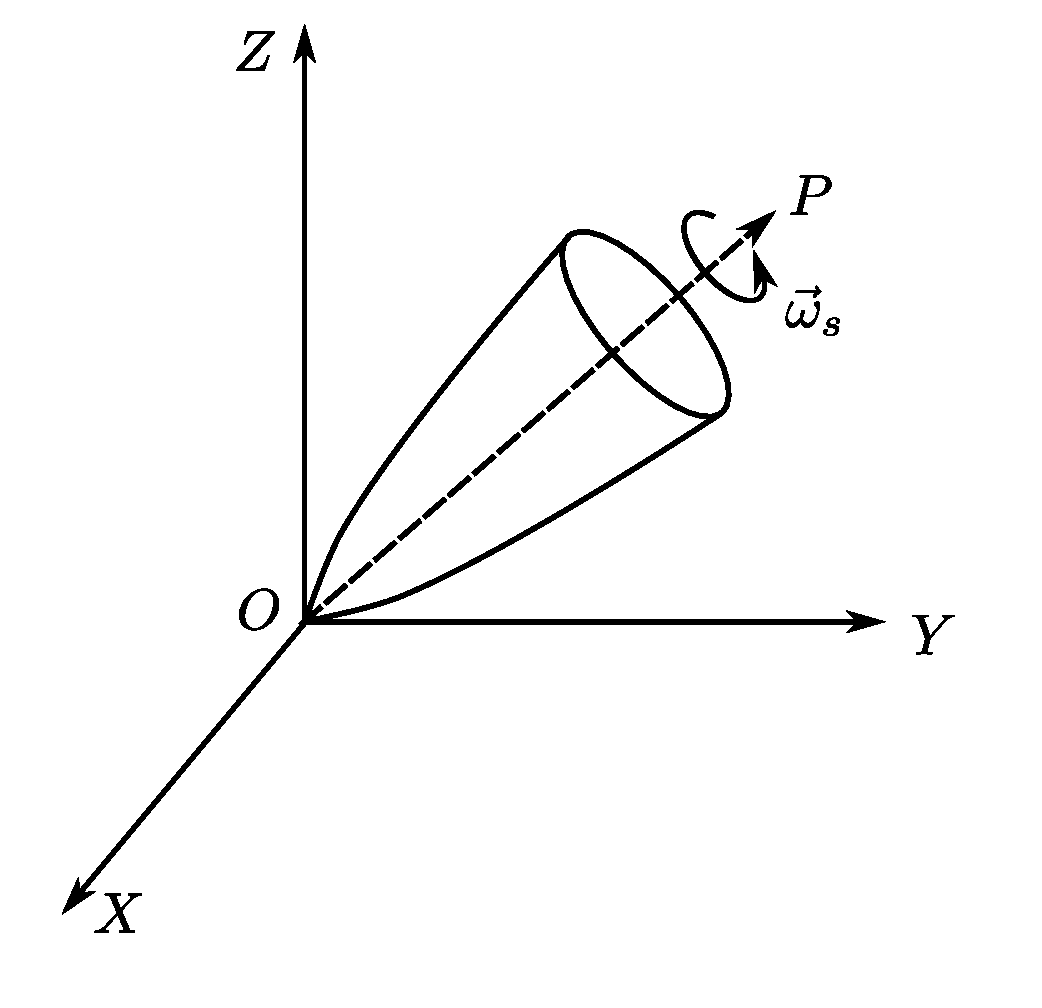
\includegraphics[width=0.4\textwidth]{spinning_top1}
%
\item* Correct answer 
\item[fraction=-50] Wrong answer  
\item[fraction=-50] Another wrong answer
\item[fraction=-50] Yet answer wrong answer
\item[fraction=-50] Answer not present here
\end{multi}
%

\begin{multi}[multiple]{Prime number}
Which numbers are prime? This question has multiple answers.
\item* 5   % or \item[fraction=50] 5
\item 6
\item* 7   % or \item[fraction=50] 7 
\item 8
\end{multi}

\begin{shortanswer}[case sensitive=true]{Einstein's name}
What was Einstein's first name?
\item Albert
\item[fraction=0, feedback={No, silly!}] Gravity
\item[fraction=0] Professor
\end{shortanswer}


%\begin{multi}{Wheel Rotation 1}
%%
%Another MCQ question is written here.
%
%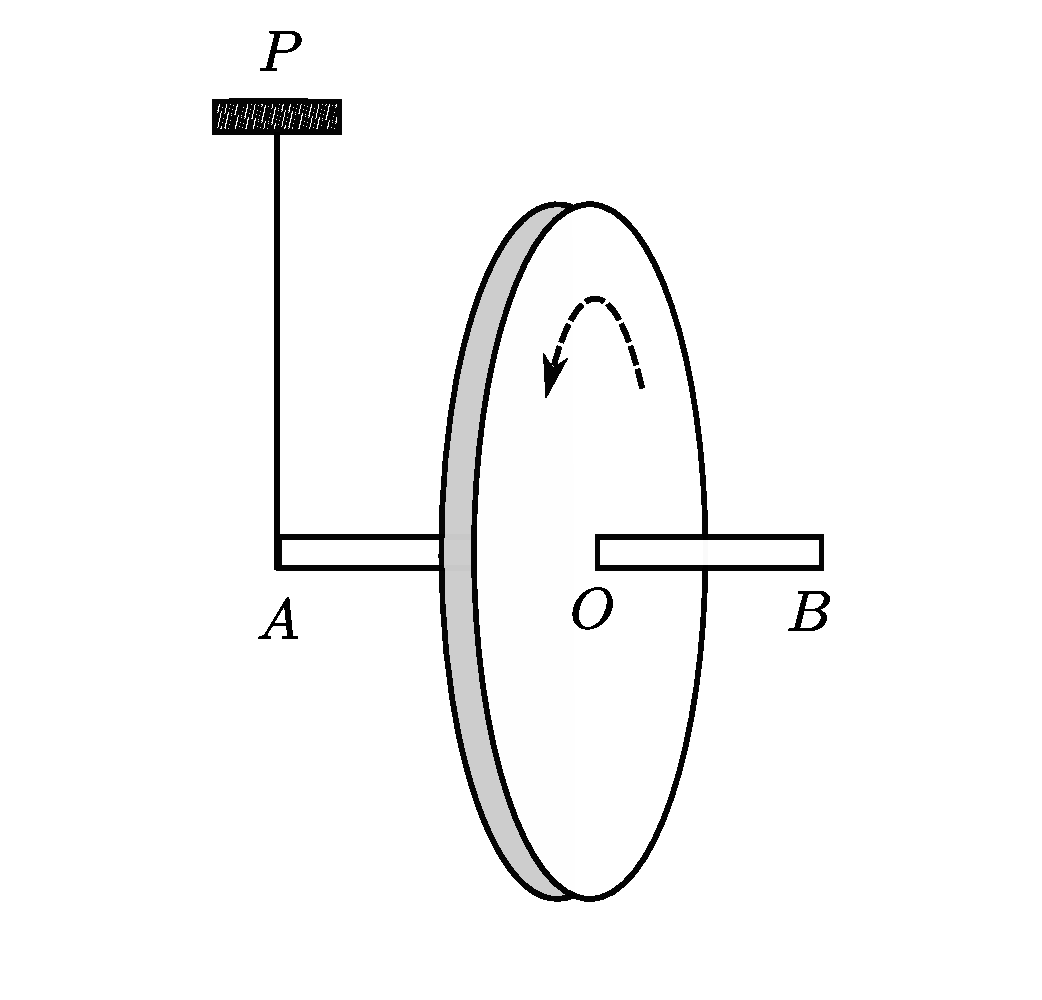
\includegraphics[width=0.4\textwidth]{wheel_rotation1}
%%
%\item* Correct answer 
%\item[fraction=-50] Wrong answer
%\item[fraction=-50] Another wrong answer
%\item[fraction=-50] Yet answer wrong answer
%\item[fraction=-50] Answer not present here
%\end{multi}
%%

\begin{numerical}{Tikz picture}
A question begins here and goes on an on. Then comes an image. 
If there is more than one correct answer, additional item's 
may be included. What is the numerical answer?

% \begin{tikzpicture}[thick,scale=0.6, every node/.style={scale=0.6}]
\begin{tikzpicture}[thick,scale=0.7]
\fill[gray!50]  (-0.75,0) circle (1cm);
\fill[gray!50]  ( 0.75,0) circle (1cm);
\draw           (-0.75,0) circle (1cm) node {$A$};
\draw           ( 0.75,0) circle (1cm) node {$B$};
\draw (-2.5,-1.5) rectangle +(5,3) node[below left]{$U$};
%     \node[below] at (0,-1.5) {Venn Diagram};
\end{tikzpicture}
%
\item 0.5
\end{numerical}

\end{quiz}

\end{document}

